\documentclass{beamer}
 
\usepackage{listings}
\usepackage[utf8]{inputenc}

 \lstdefinestyle{customc}{
  belowcaptionskip=1\baselineskip,
  breaklines=true,
  frame=L,
  xleftmargin=\parindent,
  language=C,
  showstringspaces=false,
  keywordstyle=\bfseries\color{green!40!black},
  commentstyle=\itshape\color{purple!40!black},
  tabsize=3,
  identifierstyle=\color{blue},
  stringstyle=\color{orange}
}

\lstset{escapechar=@,style=customc,numbers=left,literate={~} {$\sim$}{1}}


%TODO
% add Frederic
% add frame number
% table of contents
 
%Information to be included in the title page:
\title{Software Fault Isolation using the CompCert compiler}
\author{Alexandre Dang}
\institute{Team Celtique}
 
\begin{document}
\frame{\titlepage}
 

%%%%%%%%%%%%%%%%%%%%  SFI  %%%%%%%%%%%%%%%%%%%%
\section{Software Fault Isolation}
\label{sec:Software Fault Isolation}



\begin{frame}{Flash vulnerable plugin}
	\begin{columns}[onlytextwidth]
		\begin{column}{0.5\textwidth}
			Do you know this logo?\\
			\vspace{5mm}
			Flash is famous for its multiple vulnerabilities\\
			$\rightarrow$~consequences on Flash\\
			$\rightarrow$~but ALSO endangers your browser
		\end{column}
		\begin{column}{0.5\textwidth}
			\begin{figure}
				\centering
				
\includegraphics[width=0.7\textwidth]{images/flash.jpg}
			\end{figure}
		\end{column}
	\end{columns}
\end{frame}


\begin{frame}{Goals of Software Fault Isolation (SFI)}
	\begin{itemize}
		\item SFI aims to allow a protected program to execute dangerous modules in its own memory space without dangers. 
		\item SFI confines the execution of the dangerous modules in a reserved area called sandbox
		\item \texttt{jump} and \texttt{write} instructions are protected by runtime checks
		\item function calls to the protected programs are controlled by SFI
	\end{itemize}
\end{frame}

\begin{frame}[c]{Goals of SFI}
\begin{figure}
\centering
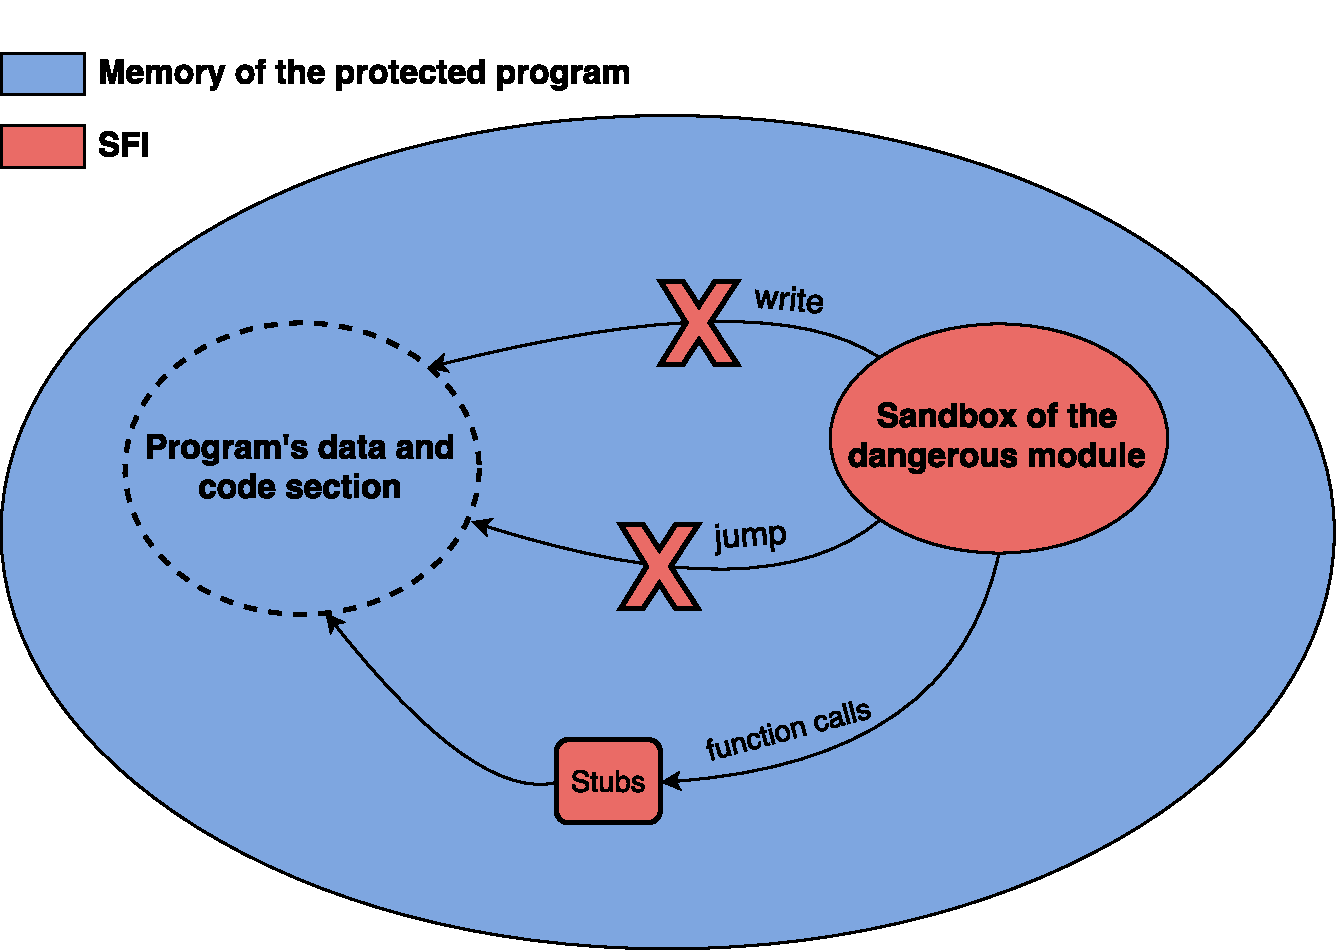
\includegraphics[width=1\textwidth]{images/sfi_principle.pdf}
\end{figure}

\end{frame}

\begin{frame}{Overview of SFI} %code gen + verifier
	SFI chain is composed of two elements:
		\begin{itemize}
			\item the \textbf{generator} transforms the assembly code of the dangerous modules in order to confine the modules in their sandbox
			\item the \textbf{verifier} checks that the SFI transformations are present and valid before loading the code in memory
		\end{itemize}
		\vspace{5mm}
		\begin{columns}
			\column{\dimexpr\paperwidth-10pt}
			\begin{center}
			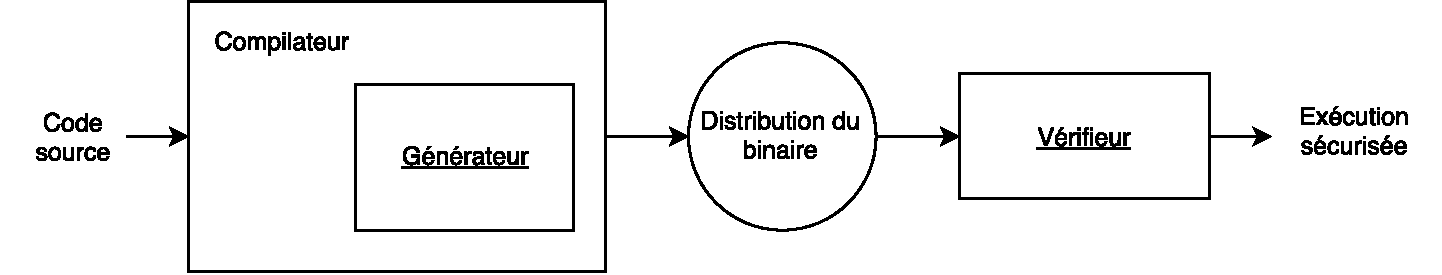
\includegraphics[width=0.95\paperwidth]{images/sfi_schema.pdf}
			\end{center}
		\end{columns}
\end{frame}

%\begin{frame}{Sandboxing}
%	Sandbox are continuous area identified by a tag. \\
%	For example the sandbox [\texttt{0xda000000}~-~\texttt{0xdaffffff}] has the tag \textbf{\texttt{0xda}}:
%	\hfill \break
%	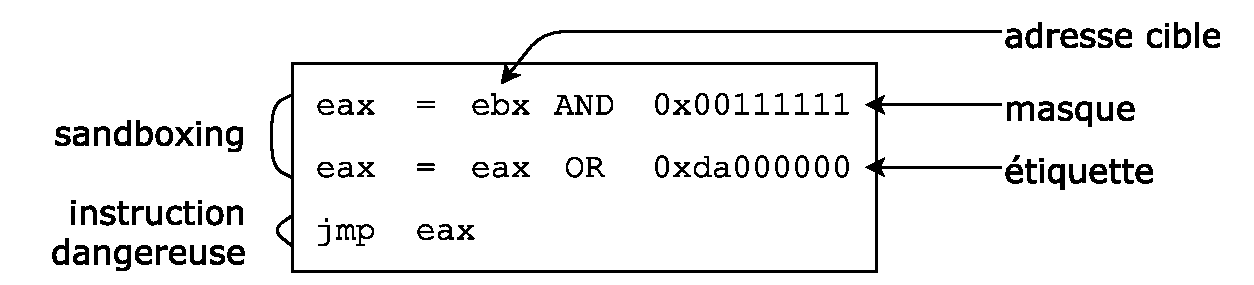
\includegraphics[scale=0.5]{images/algo_sandboxing.pdf}
%\end{frame}
%
%\begin{frame}[c]{Implementations}
%	\begin{itemize}
%		\item First implementations for RISC architecture
%		\item NativeClient, SFI for Google Chrome x86-32, x86-64 and ARM
%			\begin{itemize}
%				\item Most complete implementation of SFI
%			\end{itemize}
%		\item Portable Software Fault Isolation, implementation with the certified compiler CompCert
%			\begin{itemize}
%				\item Take advantages of the correctness of CompCert
%				\item CompCert is the compiler used for our work
%			\end{itemize}
%	\end{itemize}
%\end{frame}
%
%\begin{frame}{Pros and cons of SFI}
%	\begin{itemize}
%		\item Pros
%		\begin{itemize}
%			\item Trusted Computing Base reduced to the verifier only
%			\item Faster than protection by process separation
%		\end{itemize}
%		\item Cons
%			\begin{itemize}
%				\item Architecture dependant
%				\item Slows down the modified modules (between 5\% and 21\% depending on the implementation)
%			\end{itemize}
%	\end{itemize}
%\end{frame}
%\begin{frame}[c]{Problematics of SFI}
%	\begin{itemize}
%		\item SFI has difficulties to deal with indirect jump through return addresses
%		\item SFI is still vulnerable to Return Oriented Programing (ROP) attacks
%		\item ROP attacks are one of the most common attacks in the industry
%		\item We propose a solution to solve this issue
%	\end{itemize}
%\end{frame}

\begin{frame}[c]{Problematics of SFI}
We want to prevent attackers from using vulnerable modules to compromise our system
	\begin{itemize}
		\item SFI gives us a way to face such issue
		\item However SFI is currently lacking against Returned Oriented Programing attacks
		\item ROP attacks focus function return addresses to execute malicious code they injected
	\end{itemize}
	
\end{frame}

%%%%%%%%%%%%%%%%%%%%  ROP  %%%%%%%%%%%%%%%%%%%%
% Faire un scnario plutôt avec un mdp revele
\section{Return Oriented Programing attacks}
\label{sec:Return Oriented Programing attacks}

\defverbatim[colored]\Buffer{%
\begin{lstlisting}[tabsize=2,frame=single]
void reset_password() {
	... reset password ...
}

void foo(char* input){
	char buf[1];
	... code ...
	strcpy(buf, input);		  //Vulnerability
	... code ...
}
\end{lstlisting}}

\begin{frame}{ROP attack example (1/2)}
	\Buffer
\end{frame}

\begin{frame}[c]{ROP attack example (2/2)}
 schema	
\end{frame}

\begin{frame}[c]{Modern ROP attacks}
\begin{itemize}
	\item ROP attacks are a common kind of attack in the industry
	\item Modern ROP attacks are much more complicated 
	\item \textit{Return-to-libc} attacks uses code from the \textit{glibc} library to construct malicious code and uses return addresses to execute it
\end{itemize}
\end{frame}




%%%%%%%%%%%%%%%%%%%%  Overview  %%%%%%%%%%%%%%%%%%%%
%Contributions
%Table des matières
%Enoncer les problematiques (localisation des addresses de retour
\section{Overview of our approach}
\label{sec:Overview of our approach}

\begin{frame}[c]{Goals of our approach}
	We want to have a way to protect return addresses at runtime.
	\begin{itemize}
		\item Modifications of the memory layout in order to have an easy way to know return addresses location
		\item Code transformations which add runtime checks on the dangerous instruction in order to forbid any illegal \texttt{write} on the return addresses locations
	\end{itemize}
\end{frame}

\begin{frame}[c]{Stack structure}
	\begin{columns}
		\begin{column}{0.55\textwidth}
			\begin{itemize}
				\item Programs memory is separated into multiple area like the heap, the stack or the code section
				\item Return addresses are solely located in the stack
				\item The stack is composed of piled up frames each related to a function being executed
				\item Frames store data of their respective function
			\end{itemize}
		\end{column}
		\begin{column}{0.45\textwidth}
			\begin{figure}
			\centering
			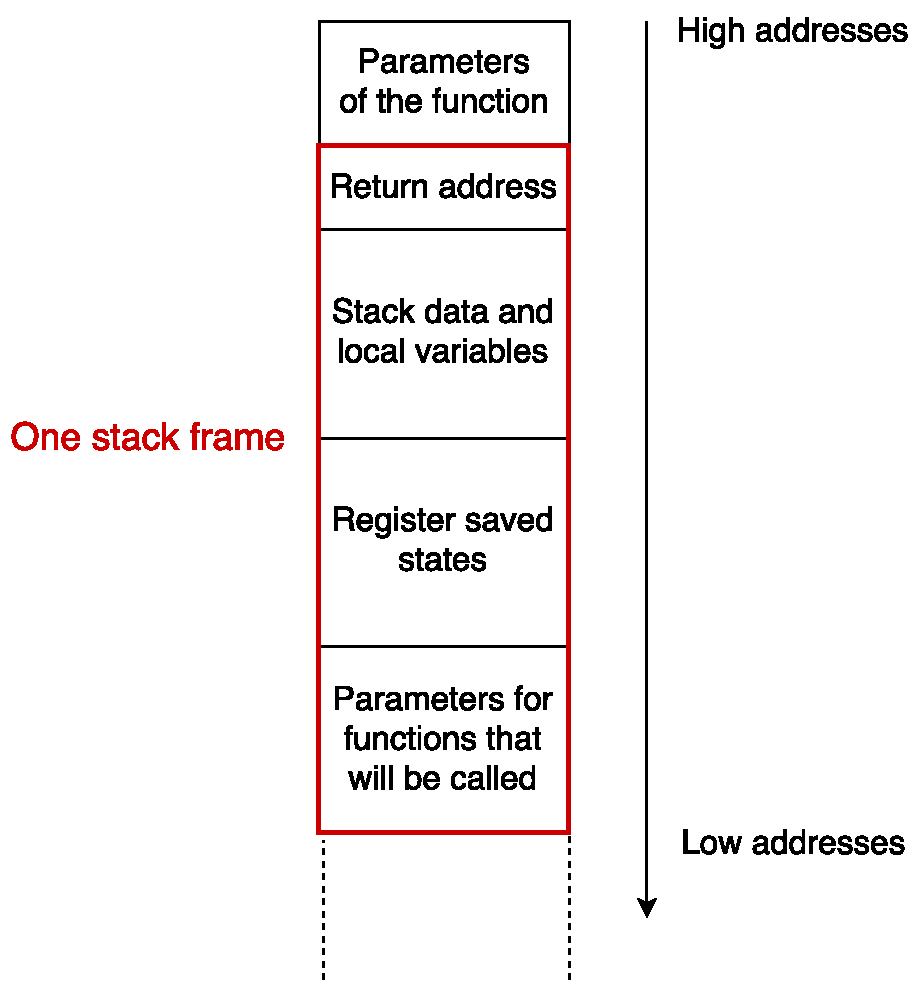
\includegraphics[height=0.75\textheight]{images/stack_layout.pdf}
			\end{figure}
		\end{column}
	\end{columns}
\end{frame}

%Faire un graphe evolutif
\begin{frame}[c]{Transformations of the stack layout}
	All the return addresses locations $a$ verify the equality $a~mod~n=0$, with $n$ a constant offset between the return addresses locations.
	\begin{enumerate}
		\item Set a constant offset $n$ between all the return addresses
		\item Align the stack
	\end{enumerate}
\end{frame}

\begin{frame}[c]{Constant offset $n$ between return addresses (1/2)}
	Constant offset $n$ between return addresses locations
	\begin{itemize}
		\item Fix frames size to $n$
		\item Pick $n$ as the biggest frame size of the previous stack
		\item Pick $n$ as a power of two
	\end{itemize}
	With this we have $a~mod~n=c$, with $c$ the location of the first return address in the stack
\end{frame}

\begin{frame}[c]{Constant offset $n$ between return addresses (2/2)}
	\begin{figure}
	\centering
	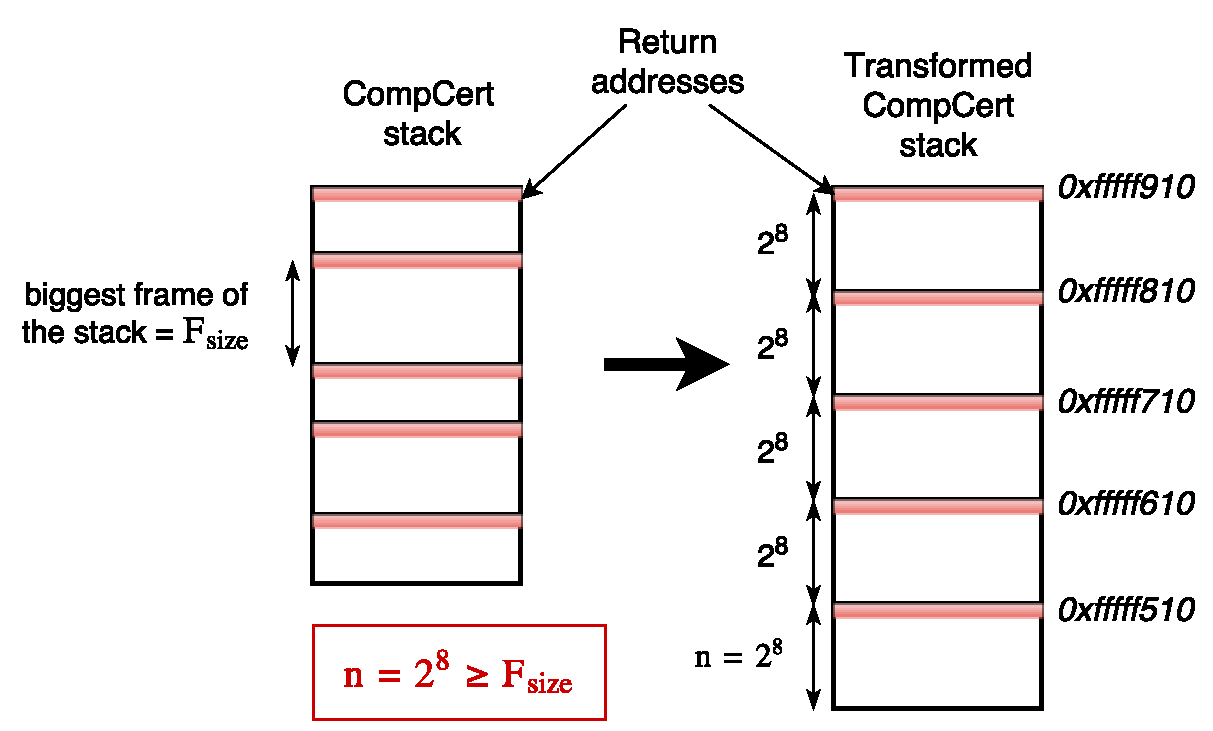
\includegraphics[width=\textwidth]{images/stack_transform.pdf}
	\end{figure}
\end{frame}

\begin{frame}[c]{Stack alignment (1/2)}
	We currently have the equality $a~mod~n=c$ but we want $a~mod~n=0$ with $a$ any return address locations  and $c$ the first return address location in the stack.
	\begin{itemize}
		\item introduce an artificial function at the beginning of the program
		\item the function align the stack as we wanted
		\item the function then calls the \textit{main} of the program
	\end{itemize}
\end{frame}

\begin{frame}[c]{Stack alignment (2/2)}
	\begin{figure}
	\centering
	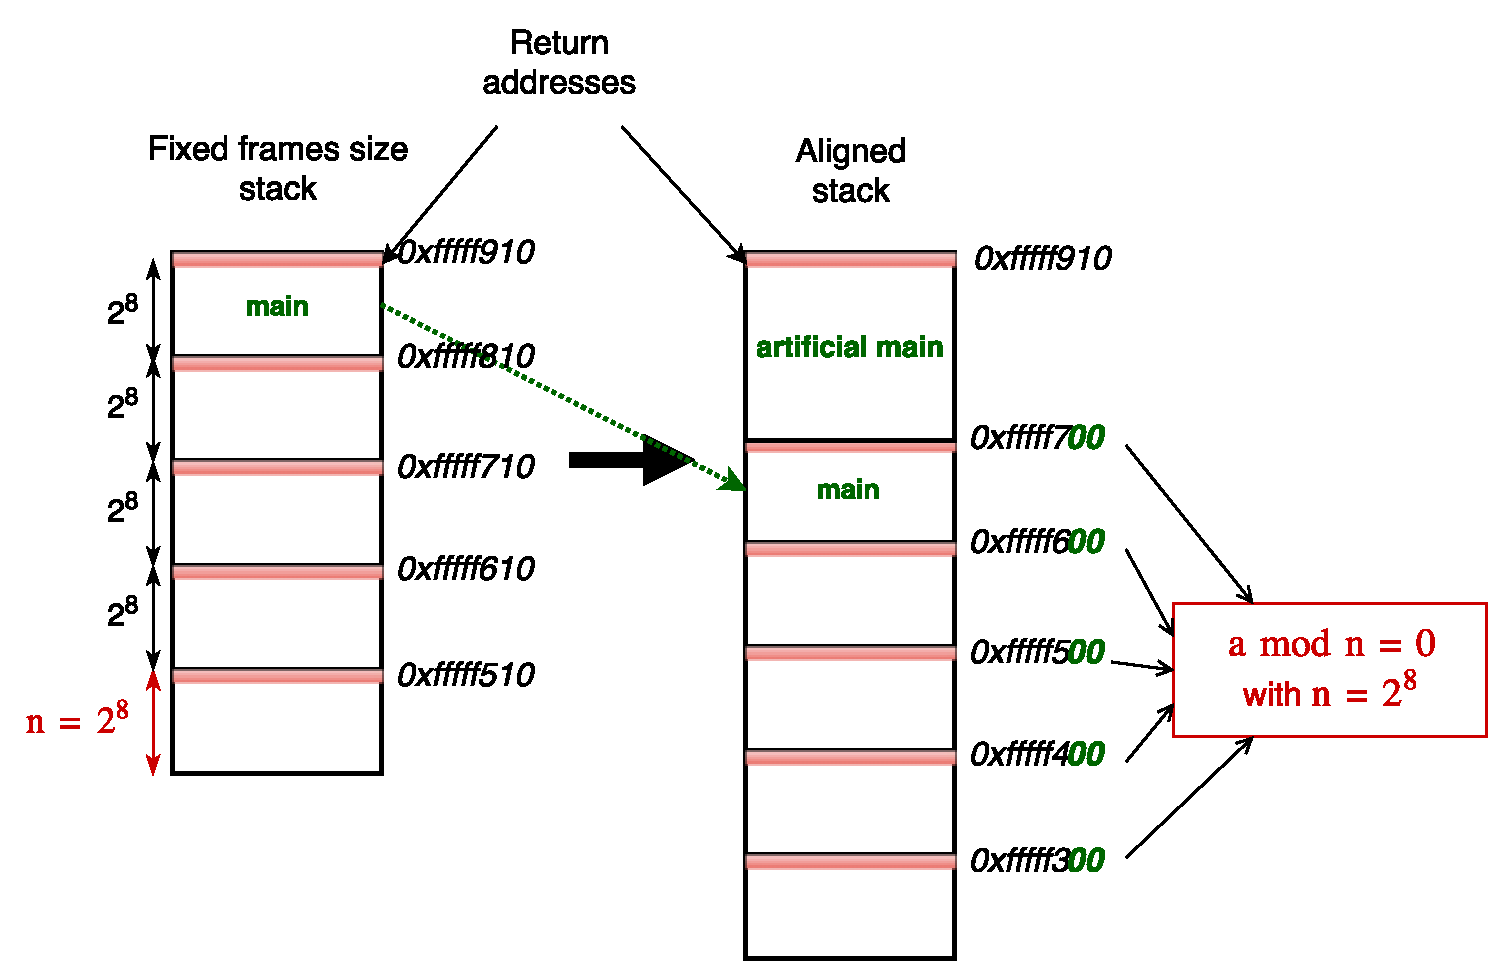
\includegraphics[width=\textwidth]{images/stack_align.pdf}
	\end{figure}
\end{frame}

\begin{frame}[c]{Code transformation}
We now know where the return addresses are located	
Prevent them from being overwritten by modifying the code
\end{frame}

%Diagramme
\defverbatim[colored]\Check{%
\begin{lstlisting}[tabsize=2,frame=single]
if (targeted_address > 0xff000000) {
	temp_var = targeted_address & (n-1);
	if (temp_var < 3) {
		Error behaviour
	} 
}
*targeted_address = value;
Continue execution...
\end{lstlisting}}

\begin{frame}[fragile]{Injection of runtime checks}
	\begin{enumerate}
		\item Check if the address is part of the stack
		\item Check if the address verifies $a~mod~n=0$
	\end{enumerate}
	\hfill \break
	\Check
\end{frame}
\defverbatim[colored]\Branchless{%
\begin{lstlisting}[tabsize=2,frame=single]
if (targeted_address > 0xff000000) {
		temp_var = targeted_address & (n-1);
		temp_var = temp_var - 3;
		temp_var = temp_var >> 31;
		temp_var = ~temp_var;
		targeted_address = temp_var & targeted_address;
}
*targeted_address = value;
Continue execution...
\end{lstlisting}}

%Diagramme
\begin{frame}{Branchless runtime checks}
	In certain cases  branchless code shows much better performance
	\Branchless
\end{frame}

\defverbatim[colored]\Inline{%
	\begin{center}
\begin{lstlisting}[tabsize=2,frame=single,linewidth=7cm]
int foo(int a) {
	asm(``\$sub 50, \%esp'');
	printf("Hello world!");
}
\end{lstlisting}
\end{center}}

\begin{frame}[c]{Implementation environment}
	CompCert
	montrer les languages concerns par les transfos
\end{frame}

%Changer le titre
\begin{frame}[c]{Conditions of our approach}
	\begin{itemize}
		\item No modifications of the stack (inline assembly)
			\Inline
		\item Need to recompile extern libraries with the same frames size
	\end{itemize}
\end{frame}

%%%%%%%%%%%%%%%%%%%%  Evaluation  %%%%%%%%%%%%%%%%%%%%
\section{Evaluation}
\label{sec:Implementation}

%Changer couleurs et mettre plus de graphes
\begin{frame}[c]{Evaluation of performance (1/2)}
	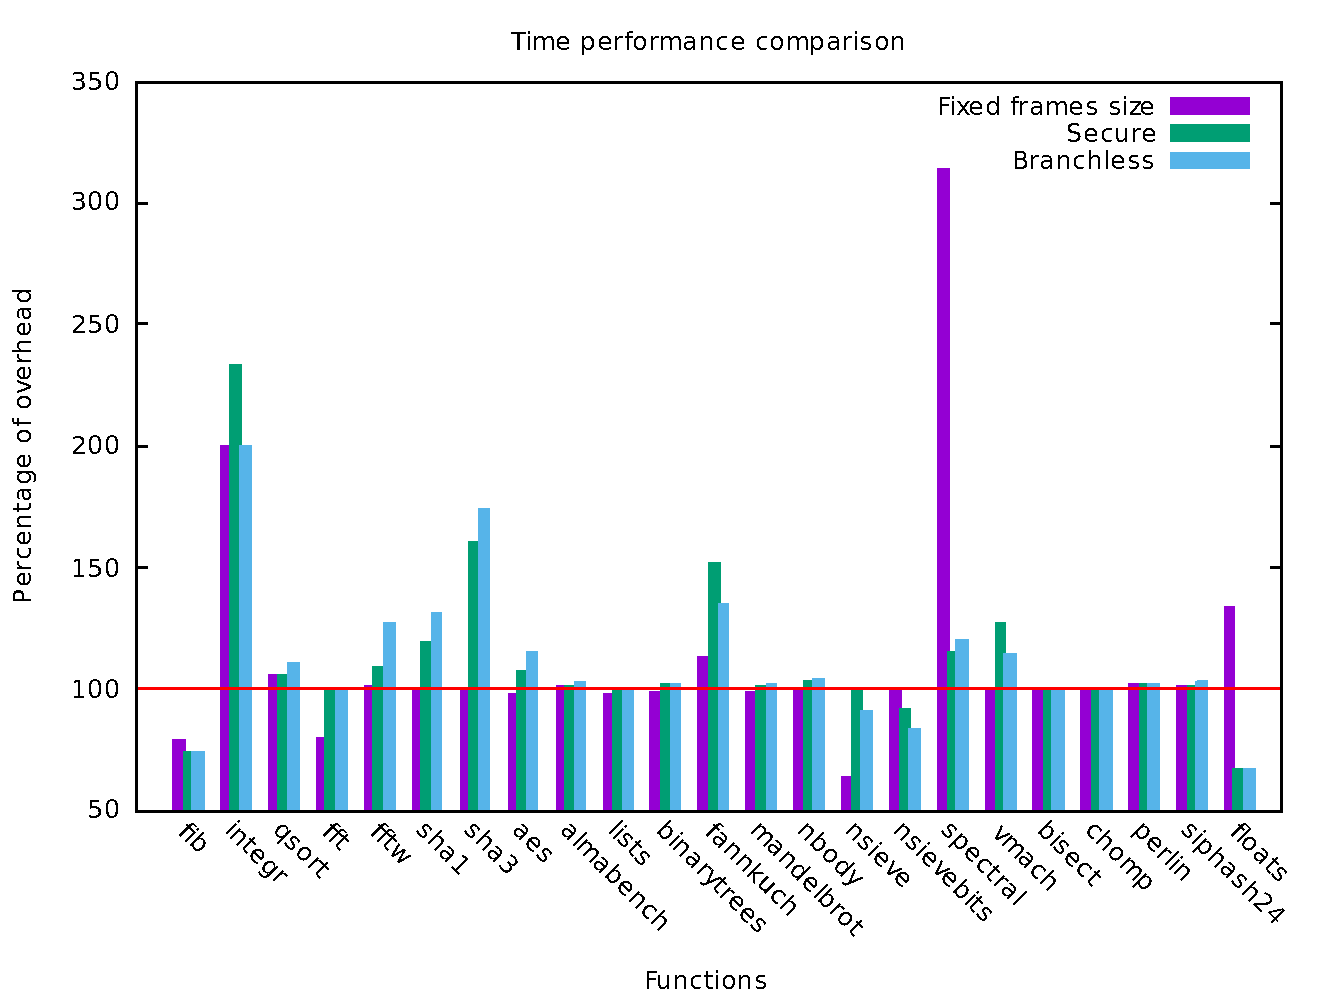
\includegraphics[width=\textwidth]{images/time_percentage_graph.pdf}
\end{frame}

\begin{frame}[c]{Conclusion}
	Prospectives
	\begin{itemize}
		\item Test our implementation against more complicated ROP attacks
		\item Reduce the number of runtime checks with static analysis
		\item Improve the performance of the runtime checks with a super-optimizer
		\item See the impact of our approach on memory consumption
	\end{itemize}
\end{frame}

 
\end{document}


